% !TeX spellcheck = fr_FR
\documentclass[12pt,a4paper]{report}
\usepackage{style/preambule_college}
\usepackage{style/preambule_personnalisation}
\usepackage{geometry}
\usepackage{amsmath}
\usepackage{graphicx}
\usepackage{tikz,tkz-tab}
\chapterFormat


\begin{document}
	\chapter[Analyse]{Aire comprise entre 2 courbes, volume d'un solide de révolution}
	\section*{Aire entre 2 courbes}
	\includegraphics{image/aire_entre_2_courbes.png}
	\vspace{1cm}
	
	Pour calculer l'aire de la surface de révolution délimitée par les courbes représentatives des 2 fonctions $f$ et $g$ continues sur $[a,b]$ et les droites d'équation $x=a$ et $x=b$, on utilise: \[ \mathcal{A}=\int_{a}^{b} \mid f(x)-g(x) \mid dx  \]
	
	Dans un premier temps nous allons résoudre l'équation $f-g=0$ pour trouver les bornes de l'aire délimitée par les 2 courbes. 
	Soit: \[f(x)=6x-x^2 \hspace{2cm} g(x)=x^2-2x \]
	$f-g=-2x^2+8x$ (appelons cette fonction $h$)
	
	$h(x)=-2x^2+8x \Leftrightarrow -2x(x-4) \rightarrow x=0$ ou $x=4$ 
	
	\vspace{1cm}
	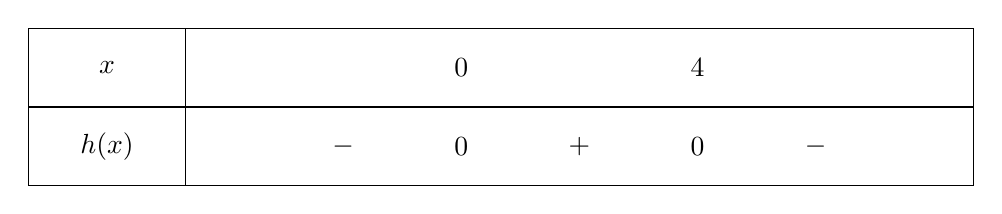
\begin{tikzpicture}
		\tkzTabInit{$x$ / 1 , $h(x)$ / 1}{ ,$0$, $4$,  }
		\tkzTabLine{ ,-, 0, +, 0, -  }
	\end{tikzpicture}
	
	Le signe de la fonction dans l'interval $[0,4]$ est positif donc: \[ \mathcal{A}= \int_{0}^{4}h(x)dx=\int_{0}^{4}(-2x^2+8x)dx=\dfrac{64}{3} \]
	
	\section*{Volume d'un solide de révolution}
	\includegraphics{image/q7_1.png}
	\vspace{1cm}
	
	\subsection*{Théorème}
	Soit une fonction $f$ continue sur [a;b]. Le volume $\mathcal{V}$ du solide de révolution dont la génératrice est la courbe représentative de $f$ entre les plans d'équations $x=a$ et $x=b$ vaut: \[ \mathcal{V}=\pi \int_{a}^{b} f^2(x)dx \]
	
	\vspace{1cm}
	\subsection*{Démonstration}
	Découpons le solide dans l'intervalle $[a;b]$ en tranche à l'aide des plans $x=x_0=a,x=x_2,...,x=x_n=b$ tous $\perp O_x$
	
	\includegraphics{image/q7_2.png}
	\vspace{1cm}
	
	Dans chaque segment $[x_{i-1};x_i]$, prenons un point arbitraire $\alpha_{i}$ et construisons un cylindre // $O_x$ dont la base est un disque de rayon $f(\alpha_{i})$; l'aire de la base d'un tel cylindre est $\pi(f(\alpha_{i}))^2$, sa hauteur est $\delta x_i =x_{i}-x_{i-1}$ et sont volume est donc $\pi(f(\alpha_{i}))^2 \delta x_i$.
	
	\vspace{1cm}
	La somme des volumes de tous les cylindres vaut $\mathcal{V}_n= \sum\limits_{i=1}^{n} \pi(f(\alpha_{i}))^2 \delta x_i$. Il s'agit d'une somme de Riemann pour la fonction $\phi (x) = \pi f^2(x)$.
	
	\medskip
	En faisant la limite de cette somme (une intégrale donc) pour $\delta_x \rightarrow 0$. Ainsi: \[ \mathcal{V}=\pi \int_{a}^{b}f^2(x)dx \]

	
	
	
	
\end{document}
